\section{Mô hình mạng nơ-ron tự mã hóa và các biến thể}

Mạng tự mã hóa là một kiến trúc mạng nơ-ron học sâu hoạt động theo cơ chế học không giám sát. Cấu trúc cốt lõi của mạng thường được thiết kế đối xứng, bao gồm hai thành phần chính: bộ mã hóa nén dữ liệu đầu vào thành một không gian ẩn có số chiều thấp hơn, và bộ giải mã khôi phục lại dữ liệu từ không gian ẩn đó sao cho đầu ra khớp nhất với tín hiệu ban đầu \cite{ref_1_6}. Trong bài toán phát hiện bất thường, cơ chế này ràng buộc mạng nơ-ron phải học cách trích xuất các đặc trưng cốt lõi và quy luật vận hành của trạng thái bình thường, đồng thời tự động loại bỏ các thành phần nhiễu không quan trọng.

\begin{figure} [H]
\centering
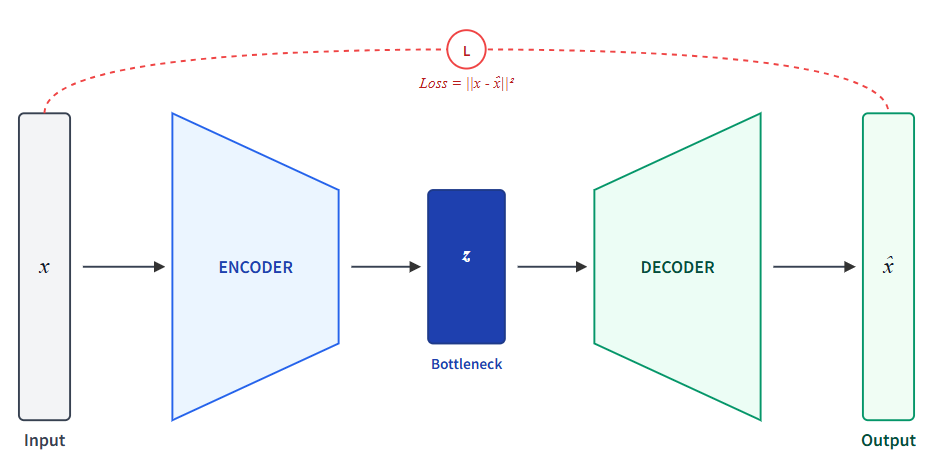
\includegraphics[width=1\linewidth]{chap1/image/Autoencoder.png}
\caption[Kiến trúc mạng nơ-ron tự mã hóa]{Kiến trúc tổng quát của mạng nơ-ron tự mã hóa.}
\label{fig:autoencoder_general}
\end{figure}

\subsection{Kiến trúc mạng Dense}

Mạng nơ-ron tự mã hóa Dense là cấu trúc cơ bản nhất của mạng tự mã hóa, trong đó mỗi nơ-ron đều được kết nối trực tiếp với toàn bộ nơ-ron ở tầng kế tiếp. Quá trình hoạt động của mạng Dense bao gồm hai giai đoạn chính. Đầu tiên, bộ mã hóa sử dụng hàm $f_{\phi}$ để ánh xạ vectơ đầu vào $x \in \mathbb{R}^d$ sang không gian ẩn $h \in \mathbb{R}^k$ (với $k < d$), như trong Phương trình \ref{eq:encoder}:

\begin{equation}\label{eq:encoder}h = \sigma(W_e x + b_e)\end{equation}

Sau đó, bộ giải mã dùng hàm $g_{\psi}$ để ánh xạ ngược từ không gian ẩn $h$ về lại không gian ban đầu, tạo ra tín hiệu phục hồi $\hat{x} \in \mathbb{R}^d$ theo Phương trình \ref{eq:decoder}:

\begin{equation}\label{eq:decoder}\hat{x} = \sigma'(W_d h + b_d)\end{equation}

Trong đó, $W_e, W_d$ là các ma trận trọng số; $b_e, b_d$ là các vectơ độ lệch (bias); và $\sigma, \sigma'$ là các hàm kích hoạt phi tuyến. Quá trình huấn luyện sẽ tối ưu hóa tập tham số $\phi$ và $\psi$ nhằm cực tiểu hóa sai số tái tạo trên dữ liệu bình thường. Với dữ liệu tín hiệu cảm biến chuỗi thời gian, hàm mất mát thường được sử dụng nhất là Sai số bình phương trung bình (Mean Squared Error - MSE):

\begin{equation}\label{eq:mse_loss}\mathcal{L}(\phi, \psi) = \frac{1}{n} \sum_{i=1}^{n} |x_i - g_{\psi}(f_{\phi}(x_i))|^2\end{equation}

Trong bài toán của đồ án, do vectơ đầu vào chỉ có kích thước 19 chiều (gồm các đặc trưng thống kê rung động và Năng lượng dải Mel - MFE\footnote{Mel-Filterbank Energy (MFE) là kỹ thuật xử lý tín hiệu âm thanh mô phỏng cách cảm nhận tần số của tai người, bằng cách nhóm các phổ tần số thu được từ biến đổi Fourier thành các dải năng lượng logarit. Chi tiết về phương pháp này sẽ được trình bày ở Mục \ref{subsec:audio_features}.}), cấu trúc Dense AE cực kỳ phù hợp. Kiến trúc nông và nhỏ gọn này giúp giải quyết hiệu quả bài toán tiết kiệm dung lượng bộ nhớ Flash và SRAM vốn rất hạn hẹp trên vi điều khiển \cite{ref_1_4}.

\subsection{Kiến trúc 1D-CNN và các giới hạn trên nền tảng nhúng}

Khác với Dense AE, mạng nơ-ron tích chập một chiều (1D-CNN) được thiết kế chuyên biệt để khai thác tính tương quan cục bộ trên dữ liệu chuỗi thời gian. Kiến trúc này sử dụng các bộ lọc (kernels) trượt dọc theo trục thời gian để trích xuất đặc trưng. Phép toán tích chập tại một vị trí $t$ với bộ lọc $w$ có kích thước $k$ được biểu diễn như Phương trình \ref{eq:conv1d}:

\begin{equation}\label{eq:conv1d}y_t = \sum_{i=0}^{k-1} w_i \cdot x_{t-i} + b\end{equation}

Về mặt lý thuyết, 1D-CNN AE rất hiệu quả trong việc nhận diện các mẫu rung động tuần hoàn hoặc các xung dị thường. Tuy nhiên, khi triển khai thực tế trên vi điều khiển, kiến trúc này bộc lộ những hạn chế lớn về mặt hiệu năng. Phép toán tích chập đòi hỏi số lượng lớn các phép nhân-cộng tích lũy (MACs), làm tăng độ trễ suy luận và tiêu tốn nhiều không gian bộ nhớ SRAM \cite{ref_1_1, ref_1_11}. Thêm vào đó, kết quả thực nghiệm của đề tài (sẽ được phân tích chi tiết tại Chương 4) còn chỉ ra một thách thức khác: sai số tái tạo của 1D-CNN AE biến động rất mạnh khi ép kiểu trọng số từ Float32 sang INT8. Điều này khiến hệ thống khó duy trì được độ tin cậy sau quá trình lượng tử hóa \cite{ref_1_1}.

\subsection{Lựa chọn kiến trúc tối ưu cho bài toán giám sát thiết bị gia dụng}

Thiết kế mô hình Trí tuệ nhân tạo tại biên (Edge AI) luôn là bài toán đánh đổi giữa độ nhạy phát hiện lỗi, độ trễ suy luận và tài nguyên bộ nhớ. Vì vậy, ở giai đoạn đầu, đồ án tiến hành so sánh ba kiến trúc mạng tự mã hóa trên môi trường mô phỏng Kaggle gồm Vanilla AE, 1D-CNN AE và LSTM AE. Các mô hình được huấn luyện trên cùng tập dữ liệu cảm biến đã tiền xử lý, sau đó được đánh giá theo sai số tái tạo, dung lượng sau lượng tử hóa INT8, độ trễ suy luận dự kiến tính toán trên Kaggle và mức ổn định khi thêm nhiễu.

Kết quả mô phỏng ban đầu xếp hạng hiệu quả theo thứ tự 1D-CNN AE, Vanilla AE và LSTM AE. Cần nhấn mạnh rằng các giá trị dung lượng và độ trễ trong giai đoạn này là số liệu dự kiến được tính toán trên Kaggle sau khi quy đổi/lượng tử hóa mô hình, chưa phải kết quả đo trực tiếp trên phần cứng. LSTM AE bị loại sớm do độ trễ suy luận dự kiến cao nhất, khoảng 129,50 ms, cùng dung lượng sau nén INT8 khoảng 368,66 KB. Vanilla AE có cấu trúc đơn giản hơn nhưng sai số tái tạo lớn nhất, với MSE đạt 0,004947, dung lượng INT8 dự kiến khoảng 375,01 KB và chỉ số bất ổn với nhiễu lên tới 793,63\%. Trong khi đó, 1D-CNN AE cho kết quả tốt nhất ở giai đoạn mô phỏng, với MSE 0,003698 và kích thước mô hình dự kiến khoảng 30,52 KB, nên ban đầu được xem là ứng viên chính cho hệ thống.

Tuy nhiên, khi chuyển sang giai đoạn triển khai trên TensorFlow Lite Micro, 1D-CNN AE bộc lộ các rào cản kỹ thuật nghiêm trọng. Kết quả suy luận giữa môi trường Python và C++ không khớp do khác biệt trong triển khai toán tử Conv1D; đầu vào dạng chuỗi làm tăng chi phí quản lý bộ đệm trên RAM; đồng thời quá trình lượng tử hóa INT8 gây rủi ro mất ổn định tham số. Từ kết quả này, đồ án chuyển sang hướng thiết kế Symmetric Dense AE kết hợp khối trích xuất đặc trưng DSP 19 chiều. Kiến trúc đối xứng giúp giảm độ phức tạp đồ thị suy luận, phù hợp hơn với giới hạn bộ nhớ của vi điều khiển Seeed Studio XIAO ESP32-S3 và trở thành kiến trúc cốt lõi cho hệ thống cuối cùng.

% ============================================================
% TÀI LIỆU THAM KHẢO TRÍCH DẪN CHO MỤC 1.2
% ============================================================
% \bibitem{ref_1_1} P. P. Ray, "A review on TinyML: State-of-the-art and prospects," 2022.
% \bibitem{ref_1_4} X. Wang et al., "Empowering Edge Intelligence: A Comprehensive Survey," 2025.
% \bibitem{ref_1_6} R. Chalapathy and S. Chawla, "DEEP LEARNING FOR ANOMALY DETECTION: A SURVEY," 2019.
% \bibitem{ref_1_10} O. K. Oyedotun and D. Aouada, "A CLOSER LOOK AT AUTOENCODERS FOR UNSUPERVISED ANOMALY DETECTION," 2022.
% \bibitem{ref_1_11} T. S. Ajani et al., "An Overview of Machine Learning within Embedded and Mobile Devices--Optimizations and Applications," Sensors, 2021.
